\documentclass{article}
\usepackage{graphicx} % Required for inserting images
\usepackage{hyperref}
\usepackage{listings}
\usepackage{xcolor}
\usepackage{float}

\graphicspath{ {./images/} }

\definecolor{codegreen}{rgb}{0,0.6,0}
\definecolor{codegray}{rgb}{0.5,0.5,0.5}
\definecolor{codepurple}{rgb}{0.58,0,0.82}
\definecolor{backcolour}{rgb}{0.95,0.95,0.92}

\lstdefinestyle{mystyle}{
    backgroundcolor=\color{backcolour},
    commentstyle=\color{codegreen},
    keywordstyle=\color{magenta},
    numberstyle=\tiny\color{codegray},
    stringstyle=\color{codepurple},
    basicstyle=\ttfamily\footnotesize,
    breakatwhitespace=false,
    breaklines=true,
    captionpos=b,
    keepspaces=true,
    numbers=left,
    numbersep=5pt,
    showspaces=false,
    showstringspaces=false,
    showtabs=false,
    tabsize=2
}

\lstset{style=mystyle}

\hypersetup{
    colorlinks=true,
    linkcolor=blue,
    filecolor=magenta,
    urlcolor=cyan,
    pdftitle={Overleaf Example},
    pdfpagemode=FullScreen,
}

\title{PhysicsSimulations}
\author{Edoardo Takanen}
\date{}

\begin{document}

    \maketitle

    \begin{center}
        \LARGE Abstract
    \end{center}

    One of the subjects I'm more interested in high school, is 100\% physics,
    we started with the concept of linear motion, then proceeding with things more \("\)complex\("\) and inarguably more interesting.
    Thus, I decided to start developing physics simulations, to challenge myself and see how many things I learn at school I can implement here.

    \newpage
    \tableofcontents

    \newpage

    \section{Introduction}\label{sec:introduction}

    These simulations will just be focusing 2D.\\
    I chose to develop this using the C++ programming language and the graphics library \href{https://www.sfml-dev.org/}{SFML}, attempting to implement by myself everything I need (collision detection, vectors etc.).
    C++ offers a very good standard library to start from as well as low level and memory management, these tools
    will be very useful for the simulations to run fast.\\
    I will also be using a library for rendering real time plots of our simulations, which can help us to analyze data while the program is running.
    The library I am talking about is \href{https://root.cern/}{ROOT},
    a powerful open-source data analysis framework coming from the CERN\@.

    \newpage

    \section{The Engine}\label{sec:the-engine}

    The first question obviously is: how can we structure our simulations' engine?\\
    I would like to follow the idea of how the \href{https://unity.com/}{Unity engine} works.
    The idea I have in mind is not only to create this physics engine, but I also want to build an API
    from which people can extend and experiment the engine.
    So the idea is to give people the tools to create something and learn, pretty much like the SFML library that I will be using.\\
    Now, let's define some basic things the engine will have:

    \begin{enumerate}
        \item Entities\\
        The basic class that let us instantiate things
        \item Objects\\
        More complex class, extends and handles specific cases for some entities (rectangles, circles, ropes etc.)
        \item Behaviors\\
        The ones that give some abilities and properties to our entities
        \item Simulation class\\
        The main class that handles entities and everything that is needed for our simulations
        \item Graphs manager\\
        The class that helps us plotting data
    \end{enumerate}

    \newpage

    We will take for granted adding vectors, which is just implementing every operator.\\
    Now we are going to look at the main function that runs a simple (and empty for now) simulation, let's write it with pseudo-code for simplicity.

    \lstinputlisting[language=C++,label={lst:main.cpp}]{./code/main.txt}

    This is a very simplified version of what we are doing every frame, I will discuss later about the
    choice of this approach.

    \newpage

    \section{Simulation}\label{sec:simulation}

    As I said above, I would like to build a usable API out of this engine.\\
    To make this, I created the Simulation class:

    \lstinputlisting[language=C++,label={lst:simulation.cpp}]{./code/simulation.txt}

    For this paper we will focus on the event functions you can see above.

    \subsection{onCreate}\label{subsec:oncreate}

    \subsection{onEvent}\label{subsec:onevent}

    \subsection{onUpdate}\label{subsec:onupdate}

    \subsection{onDrawGraphs}\label{subsec:ondrawgraphs}

    \subsection{onRender}\label{subsec:onrender}

    \newpage

    \section{Entity}\label{sec:entity}

    The entity class is the primary structure for instantiating and managing things in the simulation.

    \lstinputlisting[language=C++,label={lst:entity.cpp}]{./code/entity.txt}

    These are all the methods every entity needs.
    I will talk about behaviors later, now, before looking at the 3 main phases of each entity, I want to discuss the difference between the two events update and fixed update.

    \subsection{update vs fixed update}\label{subsec:update-vs-fixed-update}

    Basically, update runs once per frame.
    fixed-update can run once, zero, or several times per frame, depending on how many physics frames per second are set in the time settings, and how fast/slow the frame rate is.\\
    For this reason fixed update should be used when applying physics-related functions, because you know it will be executed exactly in sync with the physics engine itself.\\
    Meanwhile, update can vary out of step with the physics engine depending on how much it takes to render the frame.
    If it was used for physics, it would give different results every time!

    \subsection{update}\label{subsec:update}

    For this reason, since update is not recommended for physics functions, the function is not used, but I wanted to add it for completeness.

    \subsection{fixed update}\label{subsec:fixed-update}

    Unlike update, fixed update is very used since everything here is related to physics.
    I decided to break this out and differentiate the fixed update process into 3 phases:

    \subsubsection{beforeFixedUpdate}

    This function is the first called, and it is used to update variables like the velocity.\\
    For example, we make sure gravity is applied to our velocity each time.

    \subsubsection{checkCollisions}

    We then check for collisions for each entity in the simulation and resolve them.
    If a collision happens, we may want to apply some impulses to separate those entities.

    \subsubsection{fixedUpdate}

    Last of all, we update everything like the position or rotation.

    \subsection{render}\label{subsec:render}

    The render function is the last function called every frame.
    With this we just render our entities on the screen.

    \newpage

    \subsection{Object}\label{subsec:object}

    \newpage

    \section{Behavior}\label{sec:behavior}

    Behaviors, as I said in the introduction, are the components that give some properties to our entities.
    This is the abstract class for a behavior:

    \lstinputlisting[language=C++,label={lst:behavior.cpp}]{./code/behavior.txt}

    Behaviors can be added to entities using the \textbf{AddBehavior()} function and can be retrieved with the
    \textbf{TryGetBehavior()} function

    \newpage

    \subsection{RigidBody}\label{subsec:rigidbody}

    The RigidBody component is an implementation of physics for our entities.
    The two main functions are the followings:

    \subsubsection{Collision Detection}

    Collision detection is used to check if an object is colliding with another object
    This part will not cover the two collision detection algorithms (aabb/sat).
    I will talk about them in \ref{subsec:collisionshape}.\\
    The two types of collision detection I have implemented are:

    \begin{enumerate}
        \item Discrete
        \item Continuous
    \end{enumerate}

    \subsubsection{Discrete}

    Discrete collision detection simply uses aabb/sat algorithm and detects if there is a collision on the position where the object wants to go.

    \lstinputlisting[language=C++,label={lst:discrete.cpp}]{./code/discrete.txt}

    \paragraph{Pros and Cons}
    \begin{enumerate}
        \item \textbf{Pros}\\
        Low computational cost
        \item \textbf{Cons}\\
        Tunneling
    \end{enumerate}

    \newpage

    \subsubsection{What's tunneling?}

    \begin{figure}[H]
        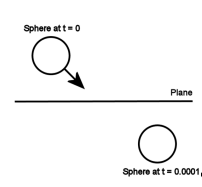
\includegraphics{TunnelingProblem}
        \centering
        \caption{The tunneling problem}
        \label{fig:tunneling}
    \end{figure}

    Tunneling is when an object moves so fast from one frame to another that
    he completely passes another object.
    \begin{enumerate}
        \item Make sure an object doesn't move too fast
        \item Increase frames per second
        \item Continuous collision detection
        \item Swept volume
    \end{enumerate}

    \subsubsection{Continuous}

    \begin{figure}[H]
        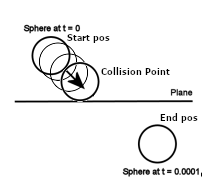
\includegraphics{ContinuousCollision}
        \centering
        \caption{Continuous collision detection}
        \label{fig:continuous}
    \end{figure}

    Continuous collision detection checks every position between start and end position, so that the computer knows the exact position where two object are colliding.

    \paragraph{Pros and Cons}
    \begin{enumerate}
        \item \textbf{Pros}\\
        Precise collision detection
        \item \textbf{Cons}\\
        Higher computation cost
    \end{enumerate}

    \subsubsection{Swept volume}

    \begin{figure}[H]
        \centering
        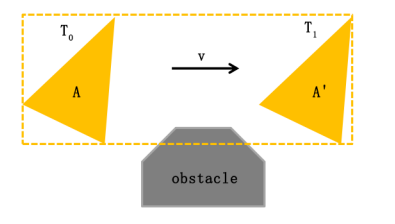
\includegraphics[width=1\linewidth]{SweptVolume}
        \caption{Swept volume}
        \label{fig:sweptvolume}
    \end{figure}

    Swept volume is the volume of the object from one frame to the next.
    With this method, we simply check the collisions considering the whole area.

    \paragraph{Pros and Cons}
    \begin{enumerate}
        \item \textbf{Pros}\\
        Low computation cost
        \item \textbf{Cons}\\
        We do not know the precise position where the collision happened
    \end{enumerate}

    \subsubsection{Velocity management}

    Velocity is used to calculate the next position of an object.\\
    \textbf{Note:} velocity can be assigned from its variable or can be updated using the \textbf{addForce()} function.\\
    Velocity is updated on fixed update, this also includes gravity.

    \newpage

    \subsection{CollisionShape} \label{subsec:collisionshape}
    \section{GraphsManager}\label{sec:graphsmanager}

\end{document}